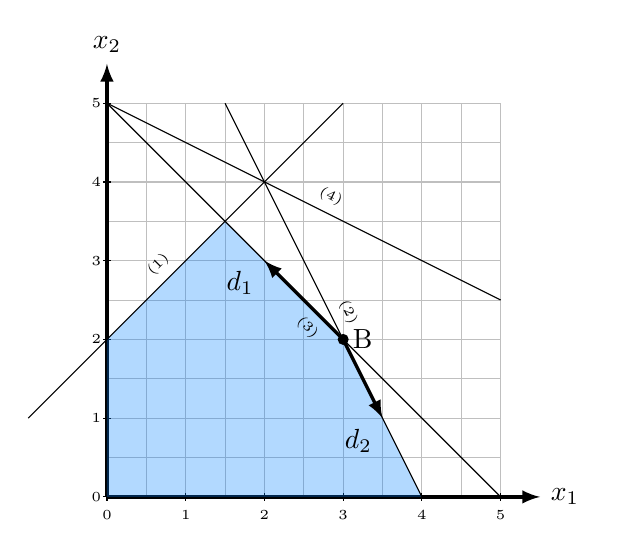
\begin{tikzpicture}
  \draw[gray!50, thin, step=0.5] (0, 0) grid (5, 5);
  \draw[very thick, -latex] (0, 0) coordinate(x1) -- (5.5, 0) coordinate(x2) node[right] {$x_1$};
  \draw[very thick, -latex] (0, 0) coordinate(y1) -- (0, 5.5) coordinate(y2) node[above] {$x_2$};
  \foreach \x in {0, ..., 5} {
    \draw (\x, 0.05) -- (\x, -0.05) node[below] {\tiny\x};
  }
  \foreach \y in {0, ..., 5} {
    \draw (-0.05, \y) -- (0.05, \y) node[left] {\tiny\y};
  }
  \fill[blue!50!cyan, opacity=0.3] (0, 0) -- (0, 2) -- (1.5, 3.5) -- (3, 2) -- (4, 0) -- cycle;  
  \draw (-1, 1) coordinate (a1) -- node[above left, sloped] {\tiny $(1)$} (3, 5) coordinate (a2);
  \draw (1.5, 5) coordinate (b1) -- node[above right, sloped] {\tiny $(2)$} (4, 0) coordinate (b2);
  \draw (0, 5) coordinate (c1) -- node[below right, sloped] {\tiny $(3)$} (5, 0) coordinate (c2);
  \draw (5, 2.5) coordinate (d1) -- node[above right, sloped] {\tiny $(4)$} (0, 5) coordinate (d2);	
  \draw[very thick, -latex] (3, 2) -- (2, 3) node[below left] {$d_1$};
  \draw[very thick, -latex] (3, 2) -- (3.5, 1) node[below left] {$d_2$};
  \coordinate (v4) at (intersection of b1--b2 and c1--c2);	
  \fill[black] (v4) node[right] {B} circle (2pt);	
\end{tikzpicture}
